\documentclass[11pt]{article}

\usepackage{fix-cm}
\usepackage{tikz}
\usetikzlibrary{shapes,backgrounds,calc,patterns}
\usepackage{amsmath,amsthm} 
\usepackage{amssymb}
\usepackage[framemethod=tikz]{mdframed}
% \usepackage{C:/Users/paulb/VSTeX/local/draculatheme}
\usepackage{mathrsfs}
\usepackage{changepage}
\usepackage{multicol}
\usepackage{mathtools}
\usepackage{hyperref}
\usepackage{slashed}
\usepackage{enumerate}
\usepackage{booktabs}
\usepackage{enumitem}
\usepackage{kantlipsum} 
\usepackage{pgfplots}
\pgfplotsset{compat=1.18}
\usetikzlibrary{decorations.markings}

\setlength{\parindent}{0pt}

\newmdenv[
  topline=false,
  bottomline=true,
  rightline=false,
  leftline=true,
  linewidth=1.5pt,
  linecolor=black, % default color, will be overridden in custom commands
  % backgroundcolor=draculabg, % Needed for Dracula theme
  % fontcolor=draculafg, % Needed for Dracula theme
  innertopmargin=0pt,
  innerbottommargin=5pt,
  innerrightmargin=10pt,
  innerleftmargin=10pt,
  leftmargin=0pt,
  rightmargin=0pt,
  skipabove=\topsep,
  skipbelow=\topsep,
]{customframedproof}

\newenvironment{proofpart}[2][black]{
    \begin{mdframed}[
        topline=false,
        bottomline=false,
        rightline=false,
        leftline=true,
        linewidth=1pt,
        linecolor=#1!40, % Custom color
        % innertopmargin=10pt,
        % innerbottommargin=10pt,
        innerleftmargin=10pt,
        innerrightmargin=10pt,
        leftmargin=0pt,
        rightmargin=0pt,
        % skipabove=\topsep,
        % skipbelow=\topsep%
    ]
    \noindent
    \begin{minipage}[t]{0.08\textwidth}%
        \textbf{#2}%
    \end{minipage}%
    \begin{minipage}[t]{0.90\textwidth}%
        \begin{adjustwidth}{0pt}{0pt}%
}{
    \end{adjustwidth}
    \end{minipage}
    \end{mdframed}
}

\newenvironment{solution}
  {\textit{Solution.}}



%%% AESTHETICS %%%
%-%-%-%-%-%-%-%-%-%-%-%-%-%-%-%-%-%-%-%-%-%-%-%-%-%-%-%-%-%-%-%-%-%-%-%-%-%-%


%%% Dimensions and Spacing %%%
\usepackage[left=0.5in,right=0.5in,top=1in,bottom=1in]{geometry}
% \usepackage{setspace}
% \linespread{1}
\usepackage{listings}
\usepackage{minted}

%%% Define new colors %%%
\usepackage{xcolor}
\definecolor{orangehdx}{rgb}{0.96, 0.51, 0.16}

% Normal colors
\definecolor{xred}{HTML}{BD4242}
\definecolor{xblue}{HTML}{4268BD}
\definecolor{xgreen}{HTML}{52B256}
\definecolor{xpurple}{HTML}{7F52B2}
\definecolor{xorange}{HTML}{FD9337}
\definecolor{xdotted}{HTML}{999999}
\definecolor{xgray}{HTML}{777777}
\definecolor{xcyan}{HTML}{80F5DC}
\definecolor{xpink}{HTML}{F690EA}
\definecolor{xgrayblue}{HTML}{49B095}
\definecolor{xgraycyan}{HTML}{5AA1B9}

% Dark colors
\colorlet{xdarkred}{red!85!black}
\colorlet{xdarkblue}{xblue!85!black}
\colorlet{xdarkgreen}{xgreen!85!black}
\colorlet{xdarkpurple}{xpurple!85!black}
\colorlet{xdarkorange}{xorange!85!black}
\definecolor{xdarkcyan}{HTML}{008B8B}
\colorlet{xdarkgray}{xgray!85!black}

% Very dark colors
\colorlet{xverydarkblue}{xblue!50!black}

% Document-specific colors
\colorlet{normaltextcolor}{black}
\colorlet{figtextcolor}{xblue}

% Enumerated colors
\colorlet{xcol0}{black}
\colorlet{xcol1}{xred}
\colorlet{xcol2}{xblue}
\colorlet{xcol3}{xgreen}
\colorlet{xcol4}{xpurple}
\colorlet{xcol5}{xorange}
\colorlet{xcol6}{xcyan}
\colorlet{xcol7}{xpink!75!black}

% Blue-Purple (should just used colorbrewer...)
\definecolor{xrainbow0}{HTML}{e41a1c}
\definecolor{xrainbow1}{HTML}{a24057}
\definecolor{xrainbow2}{HTML}{606692}
\definecolor{xrainbow3}{HTML}{3a85a8}
\definecolor{xrainbow4}{HTML}{42977e}
\definecolor{xrainbow5}{HTML}{4aaa54}
\definecolor{xrainbow6}{HTML}{629363}
\definecolor{xrainbow7}{HTML}{7e6e85}
\definecolor{xrainbow8}{HTML}{9c509b}
\definecolor{xrainbow9}{HTML}{c4625d}
\definecolor{xrainbow10}{HTML}{eb751f}
\definecolor{xrainbow11}{HTML}{ff9709}

%%% FIGURES %%%
\usepackage{graphicx}  
% \graphicspath{ {images/} }  
% \numberwithin{figure}{section}
\usepackage{float}
\usepackage{caption}

%%% Hyperlinks %%%
\usepackage{hyperref}
\definecolor{horange}{HTML}{f58026}
\hypersetup{
	colorlinks=true,
	linkcolor=horange,
	filecolor=horange,      
	urlcolor=horange,
}

\newcommand{\mysqrt}[1]{%
  \mathpalette\foo{#1}%
}
\newcommand{\dmysqrt}[1]{%
  \mathpalette\foodisplay{#1}%
}

\newcommand{\sol}[1]{
    \begin{customframedproof}[linecolor=orangehdx!75,]
        \begin{solution}
        #1
        \end{solution}
    \end{customframedproof}
}

% !TeX spellcheck = off
\newcommand{\foo}[2]{%
  % #1: math style, #2: content
  \sbox0{$#1\sqrt{#2}$}% Measure the size of the standard sqrt in the current style
  \begin{tikzpicture}[baseline=(sqrt.base)]
    \node[inner sep=0, outer sep=0] (sqrt) {$#1\sqrt{#2}$}; % Use the current math style
    \draw([yshift=-0.045em]sqrt.north east) -- ++(0,-0.5ex); % Draw the tick
  \end{tikzpicture}%
}
% !TeX spellcheck = off
\newcommand{\foodisplay}[2]{%
  % #1: math style, #2: content
  \sbox0{$#1\sqrt{#2}$}% Measure the size of the standard sqrt in the current style
  \begin{tikzpicture}[baseline=(sqrt.base)]
    \node[inner sep=0, outer sep=0] (sqrt) {$\displaystyle\sqrt{#2}$}; % Force displaystyle
    \draw[line width=0.4pt] ([yshift=-0.044em]sqrt.north east) -- ++(0,-0.5ex); % Draw the tick
  \end{tikzpicture}%
}

\newcommand{\barNotationT}[1]{\bigg|_{t = #1}}

\newcommand{\cyanit}[1]{\textit{\textcolor{cyan}{#1}}}

\newcommand{\brackett}[1]{\left\langle #1 \right\rangle}

\newcommand{\norm}[1]{\left\lVert \mathbf{#1}\right\rVert}

\newcommand{\imb}{\mb{i}}
\newcommand{\jmb}{\mb{j}}
\newcommand{\kmb}{\mb{k}}
\newcommand{\rmb}{\mb{r}}
\newcommand{\umb}{\mb{u}}

\newcommand{\vecfuc}[2]{\mb{#1}(#2)}
\newcommand{\dvecfuc}[2]{\mb{#1}'(#2)}
\newcommand{\normdvecfuc}[2]{||\mb{#1}'(#2)||}

\newcommand{\proj}{\text{proj}}

\newcommand{\mb}[1]{\mathbf{#1}}

% \renewcommand{\theenumi}{\arabic{enumi}} 
% \renewcommand{\labelenumi}{\theenumi.}

\title{Multivariable Calculus Practice Set II}
\author{Paul Beggs}
\date{\today}

%%% Custom Comands %%%
% Natural Numbers 
\newcommand{\N}{\ensuremath{\mathbb{N}}}

% Whole Numbers
\newcommand{\W}{\ensuremath{\mathbb{W}}}

% Integers
\newcommand{\Z}{\ensuremath{\mathbb{Z}}}

% Rational Numbers
\newcommand{\Q}{\ensuremath{\mathbb{Q}}}

% Real Numbers
\newcommand{\R}{\ensuremath{\mathbb{R}}}

% Complex Numbers
\newcommand{\C}{\ensuremath{\mathbb{C}}}

\newcommand{\I}{\ensuremath{\mathbb{I}}}

\newcommand{\p}{\partial}

\begin{document}

\begin{enumerate}
\setcounter{enumi}{1}
    \item (2 points) Show that \(\displaystyle \lim_{(x,y) \to (0,0)} \frac{xy^{2}}{x^{2}+y^{4}}\) does not exist.

    \sol{
        \vspace*{-1.5em}
        \begin{multicols}{2}
            \begin{itemize}
                \item \(x = 0 \) path: \(\displaystyle \lim_{(x,y) \to (0,0)} \frac{0 \cdot y^{2}}{0 + y^{4}} = \frac{0}{y^{2}} = 0\).
                \item \(y = 0 \) path: \(\displaystyle \lim_{(x,y) \to (0,0)} \frac{x \cdot 0}{x^{2} + 0} = \frac{0}{x^{2}} = 0\).
            \end{itemize}
        \end{multicols}
        \begin{itemize}
            \item \(x = y^{2}\) path: \(\displaystyle \lim_{(x,y) \to (0,0)} \frac{y^{2} \cdot y^{2}}{y^{4} + y^{4}} = \frac{y^{4}}{2y^{4}} = \frac{1}{2}\).
        \end{itemize}
        Since the limit is not the same along all paths, the limit does not exist.
    }
    \item (2 points each) Find each indicated partial derivative:
    \begin{enumerate}
        \item \(\dfrac{\partial}{\partial x} \bigl(xy^{2}\cos(x + y^{3}) - e^{xy}\bigr)\) \\

        \sol{
            \begin{align*}
                \tfrac{\partial}{\partial x} \bigl(xy^{2}\cos(x + y^{3}) - e^{xy}\bigr) &= y^{2} \tfrac{\partial}{\partial x} \bigl[x\cos(x + y^{3})\bigr] - \tfrac{\partial}{\partial x} [e^{xy}] \\
                &= y^{2} \Bigl(\cos(x + y^{3}) + x \bigl(-\sin(x + y^{3})\bigr) \Bigr) - y e^{xy} \\
                &= y^{2}\bigl(\cos(x+y^{3}) - x\sin(x + y^{3})\bigr) - y e^{xy}.
            \end{align*}
        }
        \item \(\tfrac{\partial}{\partial y} \bigl(\ln(x + y + z) - y^{2}z^{3} + x\bigr)\) \\
        
        \sol{
            \begin{align*}
                \tfrac{\partial}{\partial y} \bigl(\ln(x + y + z) - y^{2}z^{3} + x\bigr) &= \tfrac{\partial}{\partial y} \bigl[\ln(x + y + z)\bigr] - z^{3} \tfrac{\partial}{\partial y} [y^{2}] + \tfrac{\partial}{\partial y} [x] \\
                &= \tfrac{1}{x + y + z} - 2yz^{3}.
            \end{align*}
        }
        \item \(\dfrac{\p^{2}}{\p x \p y}\) \(\bigl(x^{3}y - y^{3}\tan(xy)\bigr)\) \\

        \sol{
            \begin{align*}
                \tfrac{\p^{2}}{\p x \p y} \bigl(x^{3}y - y^{3}\tan(xy)\bigr) &= \tfrac{\partial}{\partial x}\left[\tfrac{\partial}{\partial y}[x^{3}y] - \tfrac{\partial}{\partial y}\bigl[y^{3}\tan(xy)\bigr]\right] \\
                &= \tfrac{\partial}{\partial x}\left[x^{3} - (3y^{2}\tan(xy) + xy^{3}\sec^{2}(xy))\right] \\
                &= \tfrac{\partial}{\partial x}[x^{3}] - \tfrac{\partial}{\partial x}\bigl[3y^{2}\tan(xy)\bigr] - \tfrac{\partial}{\partial x}\bigl[xy^{3}\sec^{2}(xy)\bigr].
            \end{align*}
            Splitting this into 3 partial derivatives:
            \[
              \tfrac{\partial}{\partial x}[x^{3}] = 3x^{2}, \quad -\tfrac{\partial}{\partial x}\bigl[3y^{2}\tan(xy)\bigr] = -3y^{3}\sec^{2}(xy),
            \]
            with the final derivative worked out:
            \begin{align*}
                -\tfrac{\partial}{\partial x} \bigl[xy^{3}\sec^{2}(xy)\bigr] &= y^{3}\sec^{2}(xy) + \bigl[(xy^{3}) \cdot 2y\sec^{2}(xy)\tan(xy)\bigr] \\
                &= -y^{3}\sec^{2}(xy) - 2xy^{4}\sec^{2}(xy)\tan(xy).
            \end{align*}
            Combining these results, we have:
            \[
              3x^{2} - 3y^{3}\sec^{2}(xy) - y^{3}\sec^{2}(xy) - 2xy^{4}\sec^{2}(xy)\tan(xy).
            \]
            Since three terms contain a factor of \(y^{3}\sec^{2}(xy)\), we can factor this out to get:
            \[
              3x^{2} - y^{3}\sec^{2}(xy)\bigl(3 + 1 + 2xy\tan(xy)\bigr).
            \]
            Adding and simplifying further, we get:
            \[
              \boxed{3x^{2} - 2y^{3}\sec^{2}(xy)\bigl(2 + xy\tan(xy)\bigr).} 
            \] 
        }
    \end{enumerate}
    \item (3 points) Complete each of the following steps to prove that \(\displaystyle \lim_{(x,y) \to (0,0)} \frac{3x^{2}y}{x^{2} + y^{2}} = 0\). \\
    Let \(\epsilon > 0\). Choose \(\delta = \epsilon / 3\). Suppose that \((x,y)\) is chosen so that \(\| (x,y) - (0,0) \| < \delta\) and \((x,y) \neq (0,0)\).
    \begin{enumerate}
        \item Explain why \(\mysqrt{x^{2} + y^{2}} < \delta\). \\
        \sol{
           Since we have that \(\| (x,y) - (0,0) \| < \delta\), when we find the magnitude of this difference, we get:
           \[
                \boxed{\mysqrt{x^{2} + y^{2}} < \delta.}
           \]
        }
        \item Explain why \(x^{2} \leq x^{2} + y^{2}\), and thus \(\dfrac{x^{2}}{(x^{2} + y^{2})} \leq 1\). \\
        \sol{
            Because \(y^{2}\) will always be positive and \(x^{2} = x^{2}\), it must be the case that \(x^{2} \leq x^{2} + y^{2}\). Hence, when we divide both sides by \(x^{2} + y^{2}\), we get:
            \[
                \boxed{\dfrac{x^{2}}{(x^{2} + y^{2})} \leq 1.}
            \]
        }
        \item Explain why \(\dfrac{3x^{2}}{(x^{2} + y^{2})} \leq 3\). \\
        \sol{
            Since \(\dfrac{x^{2}}{(x^{2} + y^{2})} \leq 1\), multiplying both sides by 3 gives us:
            \[
                \boxed{\dfrac{3x^{2}}{(x^{2} + y^{2})} \leq 3.}
            \]
        }
        \item Explain why \(\dfrac{3x^{2}|y|}{(x^{2} + y^{2})} \leq 3|y|\). \\
        \sol{
            Similarly to the previous step, we know that since \(|y| \geq 0\), so when we multiply both sides of the inequality by \(|y|\), the inequality is unchanged.
        }
        \newpage
        \item Now, show that \(\left|\dfrac{3x^{2}y}{x^{2} + y^{2}} - 0\right| \leq 3\mysqrt{x^{2} + y^{2}}\). \\
        \sol{
            First, note that \(|y| \leq \mysqrt{x^{2} + y^{2}}\) (since \(y^{2} \leq x^{2} + y^{2}\) by the same logic in (b)). Then, recall that \(\mysqrt{x^{2} + y^{2}} < \delta\). We can multiply both sides by 3 to get \(3\mysqrt{x^{2} + y^{2}} < 3\delta\). Since \(\delta = \epsilon / 3\), when we substitute this \(\delta\) for \(\epsilon\) in our equation, we get:
            \[
                \boxed{\left|\dfrac{3x^{2}y}{x^{2} + y^{2}} - 0\right| \leq 3|y| \leq 3\mysqrt{x^{2} + y^{2}} < 3\delta = 3 \cdot \tfrac{\epsilon}{3} =  \epsilon.}
            \]
        }
        \item Conclude that whenever \((x,y)\) is in the \(\delta\)-disk centered at \((0,0)\), then \(\left|\dfrac{3x^{2}y}{x^{2} + y^{2}} - 0\right| < \epsilon\). \\
        \sol{
            Combining the previous steps, we have shown that when \((x,y)\) is in the \(\delta\)-disk centered at \((0,0)\) (i.e., \(\| (x,y) - (0,0) \|\)), we have:
            \[
              \left|\dfrac{3x^{2}y}{x^{2} + y^{2}} - 0\right| < \epsilon.
            \]
            This shows that for every \(\epsilon > 0\), we can choose a \(\delta = \frac{\epsilon}{3}\) so that whenever \(\| (x,y) - (0,0) \| < \delta\), the inequality holds. Hence, this proves that:
            \[
              \boxed{\lim_{(x,y) \to (0,0)} \dfrac{3x^{2}y}{x^{2} + y^{2}} = 0.} 
            \]
            \qed
        }
    \end{enumerate}
    \item (1 point each) Consider the contour plot of the function \(f(x,y)\) shown below. \\[0.5em]
    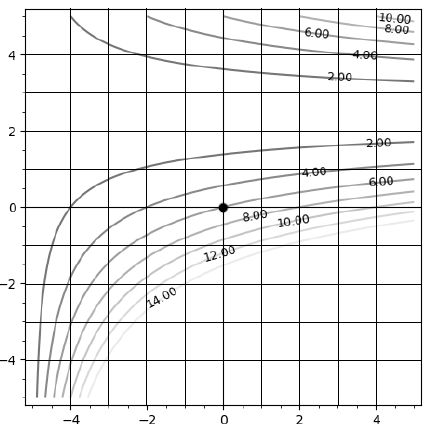
\includegraphics{contour_plot.png}
    \newpage
    Determine the sign (+, \(-\), or 0) of each of the following partial derivatives, including a \textit{brief} justification.
    \begin{enumerate}
        \item \(f_{x}(0,0)\) \\
        \sol{
            We see that \(f(0,0) = 6\), and when we move in the \(x\)-direction, the function increases slightly. Thus, \(f_{x}(0,0)\) is positive. 
        }
        \item \(f_{y}(0,0)\) \\
        \sol{
            If we move in the \(y\)-direction, the function decreases slightly towards 4. Thus, \(f_{y}(0,0)\) is negative.
        }
        \item \(f_{xx}(0,0)\) \\
        \sol{
            We can see in the plot that as we continue in the \(x\)-direction, the lines get closer together, indicating that the function is increasing. Thus, \(f_{xx}(0,0)\) is positive. 
        }
        \item \(f_{yy}(0,0)\)
        \sol{
            As we move in the \(y\)-direction, the lines get further apart, indicating that the function is decreasing. Hence, \(f_{yy}(0,0)\) is negative. 
        }
        \item \(f_{xy}(0,0)\)
        \sol{
            The function increasing in the \(x\)-direction, but when we start to move up, we can see that the lines begin to get further apart from each other. Therefore, \(f_{xy}(0,0)\) is negative.
        }
    \end{enumerate}
    \item (2 points) Find an equation of the tangent plane to \(f(x,y) = x^{2}y - \mysqrt{x} + y\) at the point \((3,1)\). \\
    \sol{
        To find the equation of the tangent plane, we need to fill out the following equation:
        \[
          z = f(a,b) + f_{x}(a,b)(x - a) + f_{y}(a,b)(y - b).
        \]
        First, we find \(z_{0}\) by plugging in the point \((3,1)\) into the function \(f\):
        \[
          z_{0} = f(3,1) = 3^{2} \cdot 1 - \mysqrt{3} + 1 = 9 - \mysqrt{3} + 1 = 10 - \mysqrt{3}.
        \]
        Thus, we must find the partial derivatives of \(f\):
        \[
          f_{x}(x,y) = 2xy - \tfrac{1}{2}x^{-1/2}, \quad f_{y}(x,y) = x^{2} + 1.
        \]
        Plugging in the point \((3,1)\) into these partial derivatives, we get:
        \[
          f_{x}(3,1) = \tfrac{12\mysqrt{3} - 1}{2\mysqrt{3}}, \quad f_{y}(3,1) = 10.
        \]
        Finally, we can plug in these values into the equation of the tangent plane to get:
        \[
          \boxed{z = 10 - \mysqrt{3} + \tfrac{12\mysqrt{3} - 1}{2\mysqrt{3}}(x - 3) + 10(y - 1).}
        \]
        \newpage
    }
    \item (2 points) For the function \(f(x,y,z) = \dfrac{x + \sin(xy)}{x^{2} + y^{2} + z^{2} + 1}\), find \(\nabla f(x,y,z)\). \\
    \sol{
        From the handout, we know that:
        \[
          \nabla f(x, y, z) = \dfrac{\partial f}{\partial x}(x, y, z)\mathbf{i} + \dfrac{\partial f}{\partial y}(x, y, z)\mathbf{j} + \dfrac{\partial f}{\partial z}(x, y, z)\mathbf{k}.
        \]
        Thus, we must find the partial derivatives of \(f\):
        \begin{align*}
            \dfrac{\partial f}{\partial x} &= \dfrac{\partial}{\partial x}\left[\dfrac{x + \sin(xy)}{x^{2} + y^{2} + z^{2} + 1}\right] \\
            &= \dfrac{(x^{2} + y^{2} + z^{2} + 1)\bigl(1 + y\cos(xy)\bigr) - 2x\bigl(x + \sin(xy)\bigr)}{(x^{2} + y^{2} + z^{2} + 1)^{2}}\\
            \dfrac{\partial f}{\partial y} &= \dfrac{\partial}{\partial y}\left[\dfrac{x + \sin(xy)}{x^{2} + y^{2} + z^{2} + 1}\right] \\
            &= \dfrac{(x^{2} + y^{2} + z^{2} + 1)\bigl(x\cos(xy)\bigr) - 2y\bigl(x + \sin(xy)\bigr)}{(x^{2} + y^{2} + z^{2} + 1)^{2}} \\
            \dfrac{\partial f}{\partial z} &= \dfrac{\partial}{\partial z}\left[\dfrac{x + \sin(xy)}{x^{2} + y^{2} + z^{2} + 1}\right] \\
            &= -\dfrac{2z\bigl(x + \sin(xy)\bigr)}{(x^{2} + y^{2} + z^{2} + 1)^{2}}
        \end{align*}
        Therefore, the gradient of \(f\) is:
        \[
        \begin{aligned}
            \nabla f(x, y, z) = \Bigg\langle& \dfrac{(x^{2} + y^{2} + z^{2} + 1)\bigl(1 + y\cos(xy)\bigr) - 2x\bigl(x + \sin(xy)\bigr)}{(x^{2} + y^{2} + z^{2} + 1)^{2}}, \\
            &\dfrac{(x^{2} + y^{2} + z^{2} + 1)\bigl(x\cos(xy)\bigr) - 2y\bigl(x + \sin(xy)\bigr)}{(x^{2} + y^{2} + z^{2} + 1)^{2}}, \, \dfrac{-2z\bigl(x + \sin(xy)\bigr)}{(x^{2} + y^{2} + z^{2} + 1)^{2}} \Bigg\rangle.
        \end{aligned}
        \]
    }
    \item (2 points) Consider the function \(f(x,y) = x^{2}y - y^{3}\). Find the directional derivative for \(f\), at \((3,4)\), in the direction of \(\mb{u} = 5\imb - 2\jmb\). \\
    \sol{
        We first find the partial derivative of \(f\) with respect to \(x\) and \(y\):
        \[
          f_{x}(x,y) = 2xy, \quad f_{y}(x,y) = x^{2} - 3y^{2}.
        \]
        Then, at the point \((3,4)\):
        \[
          f_{x}(3,4) = 2 \cdot 3 \cdot 4 = 24, \quad f_{y}(3,4) = 3^{2} - 3 \cdot 4^{2} = -39.
        \]
        Then, we find the unit vector in the direction of \(\brackett{5,-2}\): 
        \[
          \boxed{\dfrac{\brackett{24,-39} \cdot \brackett{5,-2}}{\mysqrt{29}} = \dfrac{198}{\mysqrt{29}}.}
        \]
    }
\end{enumerate}

\end{document}